\documentclass[11pt,a4paper]{book}
\usepackage{pifont}
\usepackage{color}
\usepackage{graphicx}
\usepackage{subfigure}
\usepackage{setspace}
\usepackage{fancyhdr}
\usepackage{subeqnarray}
\usepackage{ifthen}
%\usepackage[allowmove]{url}
\usepackage[hyperindex,pagebackref=true]{hyperref}
\usepackage{supertabular}
\usepackage{moreverb}
\usepackage{fancyvrb}
\usepackage{listings}
\usepackage{natbib}
\usepackage{doi}
\usepackage{longtable}
\usepackage{pdflscape}
\usepackage{psfrag}
\usepackage{makeidx}
\usepackage{palatino}
\usepackage{epsfig}
\usepackage{multirow}
\usepackage{rotating} 
%\usepackage{stmaryrd}

%Flag for htlatex compilation to html.
\newboolean{HTLatex}
\setboolean{HTLatex}{false}
\newcommand{\ifhtml}[2]{\ifthenelse{\boolean{HTLatex}}{#1}{#2}}
\newcommand{\onlypdf}[1]{\ifthenelse{\boolean{HTLatex}}{}{#1}}
\newcommand{\onlyhtml}[1]{\ifthenelse{\boolean{HTLatex}}{#1}{}}
\newcommand{\targetlabel}[1]{\hypertarget{#1}{}\label{#1}}

\usepackage{pdftricks}
\usepackage{pstricks}
\usepackage{pst-node}
\begin{psinputs}
  \usepackage{palatino}
  \usepackage{color}
  \usepackage{pst-node}
  \usepackage{graphicx}
  \usepackage{psfrag}
  \usepackage{units}
\usepackage{xspace}
\usepackage{amsfonts,amsmath,amssymb,amsthm,amsbsy,amssymb,bm}

% Place any maths notation which is also required in figures here.

% Text abbreviations.
\newcommand{\ie}{{\em{i.e., }}}
\newcommand{\eg}{{\em{e.g., }}}
\newcommand{\cf}{{\em{cf., }}}
\newcommand{\fluidity}{Fluidity\xspace}
\newcommand{\wrt}{with respect to}
\newcommand{\lhs}{left hand side}
\newcommand{\rhs}{right hand side}
\newcommand{\fluiditysourcepath}{{\tt$\textless\textless$fluidity\_source\_path$\textgreater\textgreater$}}

% Commands definining mathematical notation.

% This is for quantities which are physically vectors.
\renewcommand{\vec}[1]{{\mbox{\boldmath$#1$}}}
% Physical rank 2 tensors
\newcommand{\tensor}[1]{\overline{\overline{#1}}}
% This is for vectors formed of the value of a quantity at each node.
\newcommand{\dvec}[1]{\underline{#1}}
% This is for matrices in the discrete system.
\newcommand{\mat}[1]{\mathrm{#1}}

\renewcommand{\div}{\nabla\cdot}
\newcommand{\grad}{\nabla}
\newcommand{\curl}{\nabla\cross}

% The domain boundary.
\newcommand{\dOmega}{{\partial\Omega}}

\DeclareMathOperator{\sgn}{sgn}
\newtheorem{thm}{Theorem}[section]
\newtheorem{lemma}[thm]{Lemma}

%\newcommand\qed{\hfill\mbox{$\Box$}}
\newcommand{\re}{{\mathrm{I}\hspace{-0.2em}\mathrm{R}}}
\newcommand{\inner}[2]{\langle#1,#2\rangle}
\renewcommand\leq{\leqslant}
\renewcommand\geq{\geqslant}
\renewcommand\le{\leqslant}
\renewcommand\ge{\geqslant}
\renewcommand\epsilon{\varepsilon}
\newcommand\eps{\varepsilon}
\renewcommand\phi{\varphi}
\newcommand{\bmF}{\vec{F}}
\newcommand{\bmphi}{\vec{\phi}}
\newcommand{\bmn}{\vec{n}}
\newcommand{\bmns}{{\textrm{\scriptsize{\boldmath $n$}}}}
\newcommand{\bmi}{\vec{i}}
\newcommand{\bmj}{\vec{j}}
\newcommand{\bmk}{\vec{k}}
\newcommand{\bmx}{\vec{x}}
\newcommand{\bmu}{\vec{u}}
\newcommand{\bmv}{\vec{v}}
\newcommand{\bmr}{\vec{r}}
\newcommand{\bma}{\vec{a}}
\newcommand{\bmg}{\vec{g}}
\newcommand{\bmU}{\vec{U}}
\newcommand{\bmI}{\vec{I}}
\newcommand{\bmq}{\vec{q}}
\newcommand{\bmT}{\vec{T}}
\newcommand{\bmM}{\vec{M}}
\newcommand{\bmtau}{\vec{\tau}}
\newcommand{\bmOmega}{\vec{\Omega}}
\bmdefine{\bmphi}{\phi}
\newcommand{\pp}{\partial}
\newcommand{\kaptens}{\tensor{\kappa}}
\newcommand{\tautens}{\tensor{\tau}}
\newcommand{\sigtens}{\tensor{\sigma}}
\newcommand{\etens}{\tensor{\dot\epsilon}}
\newcommand{\ktens}{\tensor{k}}
\newcommand{\half}{{\textstyle \frac{1}{2}}}
\newcommand{\tote}{E}
\newcommand{\inte}{e}
\newcommand{\strt}{\dot\epsilon}
\newcommand{\modu}{|\bmu|}
% discretised pressure gradient operator/matrix
\newcommand{\matC}{\mat C}
% discretised divergence operator/matrix
\newcommand{\matB}{\mat B}
% Derivatives
\renewcommand{\d}{\mathrm{d}}
\newcommand{\D}{\mathrm{D}}
\newcommand{\ddx}[2][x]{\frac{\d#2}{\d#1}}
\newcommand{\ddxx}[2][x]{\frac{\d^2#2}{\d#1^2}}
\newcommand{\ddt}[2][t]{\frac{\d#2}{\d#1}}
\newcommand{\ddtt}[2][t]{\frac{\d^2#2}{\d#1^2}}
\newcommand{\ppx}[2][x]{\frac{\partial#2}{\partial#1}}
\newcommand{\ppxx}[2][x]{\frac{\partial^2#2}{\partial#1^2}}
\newcommand{\ppt}[2][t]{\frac{\partial#2}{\partial#1}}
\newcommand{\pptt}[2][t]{\frac{\partial^2#2}{\partial#1^2}}
\newcommand{\DDx}[2][x]{\frac{\D#2}{\D#1}}
\newcommand{\DDxx}[2][x]{\frac{\D^2#2}{\D#1^2}}
\newcommand{\DDt}[2][t]{\frac{\D#2}{\D#1}}
\newcommand{\DDtt}[2][t]{\frac{\D^2#2}{\D#1^2}}
% Norms
\newcommand{\Ltwo}{\ensuremath{L_2} }
% Basis functions
\newcommand{\Qone}{\ensuremath{Q_1} }
\newcommand{\Qtwo}{\ensuremath{Q_2} }
\newcommand{\Qthree}{\ensuremath{Q_3} }
\newcommand{\QN}{\ensuremath{Q_N} }
\newcommand{\Pzero}{\ensuremath{P_0} }
\newcommand{\Pone}{\ensuremath{P_1} }
\newcommand{\Ptwo}{\ensuremath{P_2} }
\newcommand{\Pthree}{\ensuremath{P_3} }
\newcommand{\PN}{\ensuremath{P_N} }
\newcommand{\PNN}{\ensuremath{P_NP_N} }
\newcommand{\Poo}{\ensuremath{P_1P_1} }
\newcommand{\PoDG}{\ensuremath{P_{1\mathrm{DG}}} }
\newcommand{\PoDGPt}{\ensuremath{P_{1\mathrm{DG}}P_2} }
\newcommand{\Pzo}{\ensuremath{P_0P_1} }
\newcommand{\Poz}{\ensuremath{P_1P_0} }
\newcommand{\PzoCV}{\ensuremath{P_0P_{1\mathrm{CV}}} }

\newcommand{\metric}{\tensor{M}}
\newcommand{\configureflag}[1]{\texttt{#1}}

% Nonlinear relaxation parameter.
\newcommand{\thetanl}{\theta_{\mathrm{nl}}}
% Implicitness parameters.
\newcommand{\thetac}{\theta_c}
\newcommand{\thetau}{\theta_{\vec{u}}}

% Notation used in timestepping.
\newcommand{\ustar}{\dvec{u}_*}
\newcommand{\unew}{\dvec{\tilde u}^{n+1}}
\newcommand{\uold}{\dvec{u}^{n}}
\newcommand{\urelax}{\vec{u}^{n+\thetanl}}
\newcommand{\pstar}{\dvec{p}_*}
\newcommand{\pnew}{\dvec{\tilde p}^{n+1}}

\newcommand{\cnew}{\dvec{\tilde c}^{n+1}}
\newcommand{\ctheta}{\dvec{c}^{n+\thetac}}
\newcommand{\cold}{\dvec{c}^{n}}
\newcommand{\cstar}{\dvec{c}_*}

\newcommand{\rhonew}{\dvec{\tilde \rho}^{n+1}}
\newcommand{\rhoold}{\dvec{\rho}^{n}}
\newcommand{\rhorelax}{\rho^{n+\thetanl}}


% Units
\newcommand{\m}[1][]{\unit[#1]{m}}
\newcommand{\km}[1][]{\unit[#1]{km}}
\newcommand{\s}[1][]{\unit[#1]{s}}
\newcommand{\invs}[1][]{\unit[#1]{s}\ensuremath{^{-1}}}
\newcommand{\ms}[1][]{\unit[#1]{m\ensuremath{\,}s\ensuremath{^{-1}}}}
\newcommand{\mss}[1][]{\unit[#1]{m\ensuremath{\,}s\ensuremath{^{-2}}}}
\newcommand{\K}[1][]{\unit[#1]{K}}
\newcommand{\PSU}[1][]{\unit[#1]{PSU}}
\newcommand{\Pa}[1][]{\unit[#1]{Pa}}
\newcommand{\kg}[1][]{\unit[#1]{kg}}
\newcommand{\rads}[1][]{\unit[#1]{rad\ensuremath{\,}s\ensuremath{^{-1}}}}
\newcommand{\kgmm}[1][]{\unit[#1]{kg\ensuremath{\,}m\ensuremath{^{-2}}}}
\newcommand{\kgmmm}[1][]{\unit[#1]{kg\ensuremath{\,}m\ensuremath{^{-3}}}}
\newcommand{\Nmm}[1][]{\unit[#1]{N\ensuremath{\,}m\ensuremath{^{-2}}}}

% Dimensionless numbers
\newcommand{\dimensionless}[1]{\mathrm{#1}}
\renewcommand{\Re}{\dimensionless{Re}}
\newcommand{\Ro}{\dimensionless{Ro}}
\newcommand{\Fr}{\dimensionless{Fr}}
\newcommand{\Bu}{\dimensionless{Bu}}
\newcommand{\Ri}{\dimensionless{Ri}}
\renewcommand{\Pr}{\dimensionless{Pr}}
\newcommand{\Pe}{\dimensionless{Pe}}
\newcommand{\Ek}{\dimensionless{Ek}}
\newcommand{\Gr}{\dimensionless{Gr}}
\newcommand{\Ra}{\dimensionless{Ra}}


\end{psinputs}

\newcommand{\note}[1]{\textbf{Note: #1}}

\usepackage{units}
\usepackage{xspace}
\usepackage{amsfonts,amsmath,amssymb,amsthm,amsbsy,amssymb,bm}

% Place any maths notation which is also required in figures here.

% Text abbreviations.
\newcommand{\ie}{{\em{i.e., }}}
\newcommand{\eg}{{\em{e.g., }}}
\newcommand{\cf}{{\em{cf., }}}
\newcommand{\fluidity}{Fluidity\xspace}
\newcommand{\wrt}{with respect to}
\newcommand{\lhs}{left hand side}
\newcommand{\rhs}{right hand side}
\newcommand{\fluiditysourcepath}{{\tt$\textless\textless$fluidity\_source\_path$\textgreater\textgreater$}}

% Commands definining mathematical notation.

% This is for quantities which are physically vectors.
\renewcommand{\vec}[1]{{\mbox{\boldmath$#1$}}}
% Physical rank 2 tensors
\newcommand{\tensor}[1]{\overline{\overline{#1}}}
% This is for vectors formed of the value of a quantity at each node.
\newcommand{\dvec}[1]{\underline{#1}}
% This is for matrices in the discrete system.
\newcommand{\mat}[1]{\mathrm{#1}}

\renewcommand{\div}{\nabla\cdot}
\newcommand{\grad}{\nabla}
\newcommand{\curl}{\nabla\cross}

% The domain boundary.
\newcommand{\dOmega}{{\partial\Omega}}

\DeclareMathOperator{\sgn}{sgn}
\newtheorem{thm}{Theorem}[section]
\newtheorem{lemma}[thm]{Lemma}

%\newcommand\qed{\hfill\mbox{$\Box$}}
\newcommand{\re}{{\mathrm{I}\hspace{-0.2em}\mathrm{R}}}
\newcommand{\inner}[2]{\langle#1,#2\rangle}
\renewcommand\leq{\leqslant}
\renewcommand\geq{\geqslant}
\renewcommand\le{\leqslant}
\renewcommand\ge{\geqslant}
\renewcommand\epsilon{\varepsilon}
\newcommand\eps{\varepsilon}
\renewcommand\phi{\varphi}
\newcommand{\bmF}{\vec{F}}
\newcommand{\bmphi}{\vec{\phi}}
\newcommand{\bmn}{\vec{n}}
\newcommand{\bmns}{{\textrm{\scriptsize{\boldmath $n$}}}}
\newcommand{\bmi}{\vec{i}}
\newcommand{\bmj}{\vec{j}}
\newcommand{\bmk}{\vec{k}}
\newcommand{\bmx}{\vec{x}}
\newcommand{\bmu}{\vec{u}}
\newcommand{\bmv}{\vec{v}}
\newcommand{\bmr}{\vec{r}}
\newcommand{\bma}{\vec{a}}
\newcommand{\bmg}{\vec{g}}
\newcommand{\bmU}{\vec{U}}
\newcommand{\bmI}{\vec{I}}
\newcommand{\bmq}{\vec{q}}
\newcommand{\bmT}{\vec{T}}
\newcommand{\bmM}{\vec{M}}
\newcommand{\bmtau}{\vec{\tau}}
\newcommand{\bmOmega}{\vec{\Omega}}
\bmdefine{\bmphi}{\phi}
\newcommand{\pp}{\partial}
\newcommand{\kaptens}{\tensor{\kappa}}
\newcommand{\tautens}{\tensor{\tau}}
\newcommand{\sigtens}{\tensor{\sigma}}
\newcommand{\etens}{\tensor{\dot\epsilon}}
\newcommand{\ktens}{\tensor{k}}
\newcommand{\half}{{\textstyle \frac{1}{2}}}
\newcommand{\tote}{E}
\newcommand{\inte}{e}
\newcommand{\strt}{\dot\epsilon}
\newcommand{\modu}{|\bmu|}
% discretised pressure gradient operator/matrix
\newcommand{\matC}{\mat C}
% discretised divergence operator/matrix
\newcommand{\matB}{\mat B}
% Derivatives
\renewcommand{\d}{\mathrm{d}}
\newcommand{\D}{\mathrm{D}}
\newcommand{\ddx}[2][x]{\frac{\d#2}{\d#1}}
\newcommand{\ddxx}[2][x]{\frac{\d^2#2}{\d#1^2}}
\newcommand{\ddt}[2][t]{\frac{\d#2}{\d#1}}
\newcommand{\ddtt}[2][t]{\frac{\d^2#2}{\d#1^2}}
\newcommand{\ppx}[2][x]{\frac{\partial#2}{\partial#1}}
\newcommand{\ppxx}[2][x]{\frac{\partial^2#2}{\partial#1^2}}
\newcommand{\ppt}[2][t]{\frac{\partial#2}{\partial#1}}
\newcommand{\pptt}[2][t]{\frac{\partial^2#2}{\partial#1^2}}
\newcommand{\DDx}[2][x]{\frac{\D#2}{\D#1}}
\newcommand{\DDxx}[2][x]{\frac{\D^2#2}{\D#1^2}}
\newcommand{\DDt}[2][t]{\frac{\D#2}{\D#1}}
\newcommand{\DDtt}[2][t]{\frac{\D^2#2}{\D#1^2}}
% Norms
\newcommand{\Ltwo}{\ensuremath{L_2} }
% Basis functions
\newcommand{\Qone}{\ensuremath{Q_1} }
\newcommand{\Qtwo}{\ensuremath{Q_2} }
\newcommand{\Qthree}{\ensuremath{Q_3} }
\newcommand{\QN}{\ensuremath{Q_N} }
\newcommand{\Pzero}{\ensuremath{P_0} }
\newcommand{\Pone}{\ensuremath{P_1} }
\newcommand{\Ptwo}{\ensuremath{P_2} }
\newcommand{\Pthree}{\ensuremath{P_3} }
\newcommand{\PN}{\ensuremath{P_N} }
\newcommand{\PNN}{\ensuremath{P_NP_N} }
\newcommand{\Poo}{\ensuremath{P_1P_1} }
\newcommand{\PoDG}{\ensuremath{P_{1\mathrm{DG}}} }
\newcommand{\PoDGPt}{\ensuremath{P_{1\mathrm{DG}}P_2} }
\newcommand{\Pzo}{\ensuremath{P_0P_1} }
\newcommand{\Poz}{\ensuremath{P_1P_0} }
\newcommand{\PzoCV}{\ensuremath{P_0P_{1\mathrm{CV}}} }

\newcommand{\metric}{\tensor{M}}
\newcommand{\configureflag}[1]{\texttt{#1}}

% Nonlinear relaxation parameter.
\newcommand{\thetanl}{\theta_{\mathrm{nl}}}
% Implicitness parameters.
\newcommand{\thetac}{\theta_c}
\newcommand{\thetau}{\theta_{\vec{u}}}

% Notation used in timestepping.
\newcommand{\ustar}{\dvec{u}_*}
\newcommand{\unew}{\dvec{\tilde u}^{n+1}}
\newcommand{\uold}{\dvec{u}^{n}}
\newcommand{\urelax}{\vec{u}^{n+\thetanl}}
\newcommand{\pstar}{\dvec{p}_*}
\newcommand{\pnew}{\dvec{\tilde p}^{n+1}}

\newcommand{\cnew}{\dvec{\tilde c}^{n+1}}
\newcommand{\ctheta}{\dvec{c}^{n+\thetac}}
\newcommand{\cold}{\dvec{c}^{n}}
\newcommand{\cstar}{\dvec{c}_*}

\newcommand{\rhonew}{\dvec{\tilde \rho}^{n+1}}
\newcommand{\rhoold}{\dvec{\rho}^{n}}
\newcommand{\rhorelax}{\rho^{n+\thetanl}}


% Units
\newcommand{\m}[1][]{\unit[#1]{m}}
\newcommand{\km}[1][]{\unit[#1]{km}}
\newcommand{\s}[1][]{\unit[#1]{s}}
\newcommand{\invs}[1][]{\unit[#1]{s}\ensuremath{^{-1}}}
\newcommand{\ms}[1][]{\unit[#1]{m\ensuremath{\,}s\ensuremath{^{-1}}}}
\newcommand{\mss}[1][]{\unit[#1]{m\ensuremath{\,}s\ensuremath{^{-2}}}}
\newcommand{\K}[1][]{\unit[#1]{K}}
\newcommand{\PSU}[1][]{\unit[#1]{PSU}}
\newcommand{\Pa}[1][]{\unit[#1]{Pa}}
\newcommand{\kg}[1][]{\unit[#1]{kg}}
\newcommand{\rads}[1][]{\unit[#1]{rad\ensuremath{\,}s\ensuremath{^{-1}}}}
\newcommand{\kgmm}[1][]{\unit[#1]{kg\ensuremath{\,}m\ensuremath{^{-2}}}}
\newcommand{\kgmmm}[1][]{\unit[#1]{kg\ensuremath{\,}m\ensuremath{^{-3}}}}
\newcommand{\Nmm}[1][]{\unit[#1]{N\ensuremath{\,}m\ensuremath{^{-2}}}}

% Dimensionless numbers
\newcommand{\dimensionless}[1]{\mathrm{#1}}
\renewcommand{\Re}{\dimensionless{Re}}
\newcommand{\Ro}{\dimensionless{Ro}}
\newcommand{\Fr}{\dimensionless{Fr}}
\newcommand{\Bu}{\dimensionless{Bu}}
\newcommand{\Ri}{\dimensionless{Ri}}
\renewcommand{\Pr}{\dimensionless{Pr}}
\newcommand{\Pe}{\dimensionless{Pe}}
\newcommand{\Ek}{\dimensionless{Ek}}
\newcommand{\Gr}{\dimensionless{Gr}}
\newcommand{\Ra}{\dimensionless{Ra}}



\makeindex
% Command to enable the labelling of the primary reference. 
% To do this use \index{term|primary}
\newcommand{\primary}[1]{\textbf{\hyperpage{#1}}}

% Cause numbering of subsubsections. 
\setcounter{secnumdepth}{5}

\definecolor{DarkBlue}{rgb}{0.00,0.00,0.55}
\hypersetup{
    linkcolor   = DarkBlue,
    anchorcolor = DarkBlue,
    citecolor   = DarkBlue,
    filecolor   = DarkBlue,
    pagecolor   = DarkBlue,
    urlcolor    = DarkBlue,
    colorlinks  = true,
    pdftitle    = {QGIS meshing plugins manual},
}

% Define date in european format
\def\today{\number\day\space\ifcase\month\or
 January\or February \or March\or April\or May\or June\or
 July\or August\or September\or October\or November\or December\fi
 \space\number\year}

\usepackage[margin=2cm]{geometry}

\newcommand{\xfig}[1]{
  \ifhtml{
    \includegraphics{#1.png}
  }{
    \input{#1.pdftex_t}
  }
}

\newcommand{\fig}[2][]{
  \ifhtml{
    \includegraphics[#1]{#2.png}
  }{
    \includegraphics[#1]{#2.png}
  }
}

\newcommand{\pdffig}[2][]{
  \ifhtml{
    % This won't work. If we ever re-enable html we'll have to deal with
    % this. 
    \includegraphics[#1]{#2.pdf}
  }{
    \includegraphics[#1]{#2.pdf}
  }
}

\usepackage{xstring}
\noexpandarg
\newcommand{\option}[1]{\texttt{\protect\StrSubstitute{#1}{/}{\slash}}}

\lstloadlanguages{[LaTeX]TeX,Python,bash,[gnu]Make,XML}

\lstset{basicstyle=\ttfamily,
  emph=anyfield,
  emphstyle=\textit,
  morekeywords={pure},
  escapeinside=`'
}
 
\usepackage{float}
 
\floatstyle{boxed}
\newfloat{example}{thp}{leg}[chapter]
\floatname{example}{Example}



\setlength{\parindent}{0.0in} \setlength{\parskip}{0.1in}

%set a few paragraph parameters
%\setlength{\parskip}{1.1ex plus 0.3ex minus 0.1ex}
%\setlength{\parindent}{0.0pt}

% Needed to fix line breaking for options
\sloppy
%\pretolerance=150
%\tolerance=300

\pagestyle{fancy}
\fancyfoot{} % No footers.
\fancyhead[RO,LE]{\thepage}
\fancyhead[RE]{\rightmark}
\fancyhead[LO]{\leftmark}
\renewcommand{\sectionmark}[1]{\renewcommand{\leftmark}{\thesection\qquad #1}}
\renewcommand{\chaptermark}[1]{\renewcommand{\rightmark}{#1}}




\begin{document}

\bibliographystyle{plainnat}

\frontmatter

\begin{titlepage}

\begin{center}

%\usefont{OT1}{cmss}{m}{n}
%\textbf{\Huge Fluidity Manual}\\
\mbox{}

\vfill

{\bfseries{\Huge
Meshing of Realistic Domains
\\}}

\vspace{5mm}

{\bfseries{\huge
Manual for the QGIS Plugins
\\}}

%\begin{figure*}[h]
%\centering
%\includegraphics[]{misc_images/manual_title.pdf}
%\end{figure*}


\vspace{80mm}

{\LARGE
Applied Modelling and Computation Group (AMCG)
\\}

\vspace{1mm}


{\LARGE
\lstinline[language=html]+http://amcg.ese.ic.ac.uk+
\\}

\vspace{10mm}

{\LARGE
Department of Earth Science and Engineering,\\
South Kensington Campus,\\
Imperial College London,\\
London, SW7 2AZ, UK
\\}

%\vspace{25mm}

%Please contact\\
%Dr M.D. Piggott\\
%(m.d.piggott@imperial.ac.uk)\\
%for additions, corrections, etc.

\vspace{40mm}


{\Large
Version 0.1 revision \input{version} (\today)
\\}

\vfill

\end{center}



\end{titlepage}

%\input{overview}
%\input{primer}

\makeatletter
% originals from book.cls
%\newcommand*\l@section{\@dottedtocline{1}{1.5em}{2.3em}}
%\newcommand*\l@subsection{\@dottedtocline{2}{3.8em}{3.2em}}
%\newcommand*\l@subsubsection{\@dottedtocline{3}{7.0em}{4.1em}}
\renewcommand\l@section{\@dottedtocline{1}{1.5em}{2.7em}}
\renewcommand\l@subsection{\@dottedtocline{2}{4.2em}{3.6em}}
\renewcommand\l@subsubsection{\@dottedtocline{3}{7.8em}{4.5em}}

% new command to add Word-style comments to text
\newsavebox{\marginbox}% contains the contents of the comment environment
\let\comment\relax% removes and previous definition of \begin{comment}
\let\endcomment\relax% removes any previous definition of \end{comment}
\newenvironment{comment}{
  \begin{lrbox}{\marginbox}
  \begin{minipage}{\marginparwidth}
  \footnotesize
  }{
  \end{minipage}
  \end{lrbox}
  \marginpar{\usebox{\marginbox}}
  }

\makeatother

{ \setlength{\parskip}{0pt} \tableofcontents \listoffigures }

\newpage \clearpage \thispagestyle{plain}

\mainmatter

%\setcounter{chapter}{1}
\chapter{Getting started}
\label{chptr:getting_started}

\section{Introduction}
\label{sect:introduction}
One of the first steps in computational simulations of continua is the specification of the domain, and its tessellation into non-overlapping cells or elements. In the context of computational ocean fluid dynamics, the domain is typically bound by \emph{open boundaries}, the \emph{free surface}, \emph{ocean floor} and perhaps an \emph{ice-shelf} as identified in figure \ref{fig:typical_ocean_modelling_domain}. In practice, domain boundaries are frequently extracted by topography/morphology data such as the data shown in figure \ref{fig:rtopo_atlas} for the region around the South Pole. The panels of figure \ref{fig:rtopo_atlas} show contour plots of a subset of the data available in the RTOPO dataset \citep{timmermann_et_al:2010}: The region bathymetry(left panel), surface elevation (right panel) and filled contours that characterise the surface of the region in terms of shelf-ice, sea or land.
\begin{figure}[htb!]\begin{center}
%\scalebox{0.6}{\includegraphics{}}
\caption[A typical domain encountered in computational ocean fluid dynamics.]{A typical domain encountered in computational ocean fluid dynamics.}
\label{fig:typical_ocean_modelling_domain}
\end{center}\end{figure}
\begin{figure}[htb!]\begin{center}
\scalebox{1.0}{\includegraphics{meshing_images/rtopo_maps.pdf}}
\caption[Data from the the R-TOPO Antarctica atlas.]{Three data-sets from the R-TOPO Antarctica atlas. Left: Bathymetry. Centre: Identification of surface cover. Right: surface elevation. All plots in stereographic projection}
\label{fig:rtopo_atlas}
\end{center}\end{figure}
\par
Usually the domain boundary specification can be essentially reduced to an operation in two-dimensions alone: The equations solved are two-dimensional (\eg the shallow-water equations) or, as is the case in \fluidity, the two dimensional mesh is projected to the top and bottom surfaces of the domain and a three-dimensional mesh is created during an \emph{``extrusion''} procedure, as conveyed in figure \ref{fig:2d_domain_and_extrusion}. Then the process of domain specification reduces to the specification of shorelines, grounding lines and open boundaries on a reference surface such that a closed domain is formed, as shown in figure \ref{fig:2d_domain_and_extrusion}. 
\begin{figure}[htb!]\begin{center}
%\scalebox{0.6}{\includegraphics{}}
\caption[A two dimensional mesh and schematic of the extrusion procedure.]{Left: A two-dimensional mesh. Right: Schematic conveying the extrusion procedure.}
\label{fig:2d_domain_and_extrusion}
\end{center}\end{figure}
\par
Another essential part of mesh generation for ocean modelling is the specification of mesh size. Smaller elements are typically required in shallow regions, near the coastlines (in order to accurately represent the aforementioned complex boundaries), in areas of steep bathymetry or simply in regions of interest (\eg tidal farm installations). Figure \ref{} shows the two-dimensional field of the mesh size metric as filled contours.
\par
It is clear from figures \ref{fig:typical_ocean_modelling_domain}, \ref{fig:2d_domain_and_extrusion} and \ref{fig:rtopo_atlas} that shorelines, grounding lines and the ocean floor are very complex: They are fractal-like geometries, characterised by a large range of scales. However, the extraction of boundaries and production of mesh size metric maps can be easily handled through \emph{Geographic Information Systems (GIS)} software. GIS software is capable of importing a large range or data-formats frequently used to represent morphology (\eg netCDF, png) or port \& coastline surveys (\eg shapefiles), such as shown in figure \ref{fig:rtopo_atlas}. Tools for processing such data are also provided, already facilitating some of the operations mentioned above.
Once the domain has been fully defined and the mesh size has been specified, this information can be passed to a mesh generator to produce the desired mesh. We have thus identified two essential components in a mesh generation procedure of ocean and coastal domains: First a component that can be used for processing of geographical information. Second a robust mesh generator. A typical work-flow in mesh generation of ocean and coastal domains is shown in figure \ref{fig:main_components}, showing the two aforementioned components. On the left side, the input data such as bathymetry is identified by the green ellipse. The red ellipse identifies the interaction with the user in order to extract and plot boundaries and the desired mesh-size metric. Note that the interaction of the user and the GIS software and the communication of information between the GIS software and the meshing software is accomplished through the \emph{meshing plug-ins}, the third component of the work-flow, and the subject of this manual.


\begin{figure}[htb!]\begin{center}
\scalebox{1.0}{\includegraphics{meshing_images/ocean_mesh_generation_overview.pdf}}
\caption[The usual meshing workflow.]{A work-flow typical in mesh generation of ocean and coastal domains.}
\label{fig:main_components}
\end{center}\end{figure}
\par
As figure \ref{fig:main_components} shows the software of choice is Quantum GIS and Gmsh:
\begin{enumerate}
  \item{\emph{Quantum GIS} (QGIS, \url{http://www.qgis.org/}):} is a user friendly Open Source Geographic Information System (GIS) licensed under the GNU General Public License. QGIS is an official project of the Open Source Geospatial Foundation (OSGeo). It runs on Linux, Unix, Mac OSX, Windows and Android and supports numerous vector, raster, and database formats and functionalities. A very attractive feature of QGIS is its extensibility via python ``plug-ins''. This method is used here to provide the interactions described above withthe help of figure \ref{fig:main_components} as a part of QGIS.
  \item{\emph{Gmsh} (\url{http://www.geuz.org/gmsh/}):gmsh licence and quick description}
\end{enumerate}
The remainder of this manual, bla bla bla....



\section{Obtaining and using Quantum GIS}
\label{sect:obtaining_and_using_qgis}

\subsection{Obtaining Quantum GIS}
\label{sec:install}
On the Ubuntu Linux distribution {Q}{G}{I}{S} is available through the Ubuntu package system and can be installed by typing: 

\begin{example}
\begin{lstlisting}[language=bash]
  wajig install qgis
\end{lstlisting}
\end{example}

To obtain useful supporting packages, add the UbuntuGIS repository,  see

\url{https://wiki.ubuntu.com/UbuntuGIS}.

This can be done with the following:

\begin{example}
  \begin{lstlisting}[language=bash]
  $ sudo add-apt-repository ppa:ubuntugis/ppa 
  $ wajig update
\end{lstlisting}
\end{example}

and install the following:

\begin{example}
  \begin{lstlisting}[language=bash]
  $ wajig install blender qgis python-shapely inkscape grass
    qgis-plugin-grass thuban gmt gpsbabel gpx2shp gpsd 
    gpsd-clients gpsdrive gpsman avce00 e00compr cgi-mapserver
    mapserver-bin perl-mapscript php5-mapscript python-mapscript
    postgis python-gdal proj libterralib1c2a
\end{lstlisting}
\end{example}

Note that on Precise, you need to replace the last library \emph{libterralib1c2a} with \emph{libterralib}.

\subsubsection{Direct Download}

To either use a newer version of the software or to simply gain access to
QGIS without installing the system's packages, a pre-compiled QGIS
client can be downloaded from the QGIS website at:

\url{http://hub.qgis.org/projects/quantum-gis/wiki/Download}

This download page has pre-compiled client software for 32-bit and 64-bit
Windows, Linux, and Mac OS X. Administrative privileges may be needed on the
computer to install the software.

\subsubsection{Supporting Packages}
In order for the \emph{Mesh NetCDF} and \emph{Define Boundary ID's} plugins to work, the Python package `Shapely' will need to be installed. This package carries out vector operations such as intersections when working with Shapefile polygon objects. This package is listed in the large install block in Section~\ref{sec:install}.

\subsection{Running QGIS}

On a Ubuntu system, QGIS can be run by typing 'qgis' into a
terminal. Note that when running it entirely locally it can be heavy on both CPU
and graphics card which in turn means it is heavy on battery life if
intensively used on a laptop.

On a Mac the QGIS application will probably have been put in the
Applications directory during the install procedure, and it can be run from
there.

No information is available about how to run QGIS in Windows. 

which should return something like:

\begin{example}
  \begin{lstlisting}[language=bash]
  $ which qgis
  /usr/bin/qgis
\end{lstlisting}
\end{example}

\subsection{Using QGIS}
% Drawing polygons.
% Difference operation.
% Extracting contour. GUI or Polygonize.
% Removing parts of the domain.

\subsection{Reading in data}

%See fig.~\ref{fig:multiple1} and also in particular fig.~\ref{fig:calc}.


\subsubsection{Opening files}

\subsubsection{Reading in fields}


\section{Obtaining and using Gmsh}
\label{sect:obtaining_and_using_gmsh}

\section{Obtaining the plugins}
\label{sect:obtaining_the_plugins}
Please download the qgis-plugins-meshing Ubuntu package which is available in the following PPA:

\begin{example}
  \begin{lstlisting}[language=bash]
  ppa:meshing/release
\end{lstlisting}
\end{example}

(which depends on packages in ppa:ubuntugis/ppa)

Commands required:
\begin{example}
  \begin{lstlisting}[language=bash]
  sudo add-apt-repository ppa:ubuntugis/ppa
  sudo add-apt-repository ppa:meshing/release
  sudo apt-get update
  sudo apt-get install qgis-plugins-meshing
\end{lstlisting}
\end{example}

If the final command fails, please download the package manually from
\url{http://amcg.ese.ic.ac.uk/~asc/public/qgis-plugins-meshing_1.9_all.deb}
and install with

\begin{example}
  \begin{lstlisting}[language=bash]
  sudo dpkg -i qgis-plugins-meshing_1.9_all.deb
\end{lstlisting}
\end{example}

(there is a fix for Precise, which is currently being processed by Launchpad).


\chapter{The Meshing Plugins}
Meshing to realistic domains is achieved through the following four plugins:
\begin{itemize}
\item \emph{RasterCalc} can be used to perform calculations on raster fields such as addition, integration, divergence etc. and is able combine raster fields - see Section~\ref{sec:rasterCalc}. 
\item \emph{Rasterise Polygons} creates NetCDF raster layers from user defined Shapefile polygons; the extent of raster is the same as the defined background raster layer - see Section~\ref{sec:rasterisePolygons}. 
\item \emph{Define Boundary ID's} allows the labelling of boundaries so that seperate boundary conditions can be applied to the generated Geo file in Fluidity - see Section~\ref{sec:defineBoundaryIDs}. 
\item \emph{Mesh NetCDF} generates a mesh from a Shapefile or Geo file using an optional NetCDF file as a mesh-size metric - see Section~\ref{sec:meshNetCDF}.
\end{itemize}

\textbf{It is strongly recommended to run QGIS from the Terminal to allow the viewing of status prints incorporated into the plugins and to monitor current operations.}

\subsection{RasterCalc}
\label{sec:rasterCalc}
\begin{spacing}{0}
	\small
	\raggedleft{ Plugin Source: \url{http://gis-lab.info/qa/rastercalc.html}
	\\Plugin Amended by: Elliot Lynch, Varun Verma
	\\Documentation Written by: Varun Verma, \url{http://gis-lab.info/qa/rastercalc.html}
	}
\end{spacing}
\normalsize
\vspace{3mm}
This plugin can be used to perform raster calculations with multiple raster layers in QGIS, with the result writen to a single output file. This is a functional raster calculator which is implemented as an extension to Quantum GIS.
\subsubsection{Usage}

\begin{figure}[h!]
  \centering
  \fig[width=.7\textwidth]{meshing_images/rc_window}
  \caption{Raster Calulator}
  \label{fig:rc_window}
\end{figure}
The RasterCalc window (Figure~\ref{fig:rc_window}) contains the following elements:
\begin{description}
	\item[\hspace{5mm} 1. ] List of rasters loaded in the project. Rasters are grouped by size.
	\item[\hspace{5mm} 2. ] Channel list raster filled automatically when a raster is selected.
	\item[\hspace{5mm} 3. ] Buttons to quickly add features. There is also a drop-down for expression templates.
	\item[\hspace{5mm} 4. ] Entry area, which is displayed as a formatted expression. Supports copying and pasting text.
	\item[\hspace{5mm} 5. ] Message line that displays errors, warnings and information.
	\item[\hspace{5mm} 6. ] Reset button and to load/save equations.
	\item[\hspace{5mm} 7. ] Drop-down list to control the data type for pixel values in the output raster.
	\item[\hspace{5mm} 8. ] Field to enter the name of the resulting file.
	\item[\hspace{5mm} 9. ] Check box that allows the resultant raster file to be loaded into the map Canvas.
	\item[\hspace{5mm} 10.] Buttons to exit the plugin or preform the calculation.
\end{description}

RasterCalc supports the use of all Numpy array operations. Format expressions - traditional, as in mathematics, there are support brackets, including attachments. Raster names must be enclosed in square brackets (`[]'), after the name of the raster through a `dog' (`@') must specify the channel number. Inserting a raster into the expresion is performed by double-clicking on the appropriate list item bitmap. The inserted raster will automatically use the 1st channel (and will be added to the channel list). 
Some common operations are available in the form of `templates'. After selecting one of these `templates' from the drop down list it is inserted into the input area, and filled out with available raster layers.
Durring the input process, the expression is verifide with errors displayed in the message line.  Detected errors will result in the "calculate" button being disabled. 
\vspace{5mm}
The functions which are assigned to private buttons are as follows:
	\begin{itemize}
		\item Arithmetic operations (+, -, *, /).
		\item Trigometric functions (sin, cos, tan, asin, acos, atan).
		\item The natural logarithm (log), the exponent (exp) and exponentiation (\^{}).
		\item Insert the brackets mark the capture channel.
	\end{itemize}
The following functions have been implemented, but do not have buttons due to fast insertion (ie, you must manually type these functions to perform them): 
	\begin{itemize}
		\item Comparison operators ($<$,$>$,=, !=, $<$=,$>$=).
		\item Conditionals (lt - less than, gt - greater than, eq - equal, ne - not equal, le - less than or equal, ge - greater than or equal to).
	\end{itemize}
\vspace{5mm}
Comparison operators can compare pixel-channel raster with some value or another channel of the same or any other raster. Comparisons will screen in which all pixels satisfying receive a value of 1, and all others, respectively, 0. Conditional statements are a further development of comparison operators. The operator takes three arguments: 
	\begin{enumerate}
		\item Screen, which is compared.
		\item Value with which to compare. 
		\item Value used for the replacement values.
	\end{enumerate}
The second and third arguments can be numbers, arbitrary channel raster (in this case, the per-pixel comparison and/or replacement) or an expression. 

\begin{figure}[h!]
  \centering
  \fig[width=.2\textwidth]{meshing_images/tooltip}
  \caption{ToolTip}
  \label{fig:tooltip}
\end{figure}


The function buttons have a tool tip as shown in Figure~\ref{fig:tooltip} to allow the user to know which function would be performed by each individual button. The definition of the non-trivial functions which can be performed on the raster layers are explained below:
	\begin{itemize}
		\item intS: Surface Integral (Sum of intx and inty).
		\item intF: Integration of a pair of rasters (Fields).
		\item inty: Integrate with respect to the vertical parameter; longitude or y axis.
		\item intx: Integrate with respect to horizontal parameter; latitude or x axis.
		\item ddy: Differentiate with respect to vertical parameter; longitude or y axis.
		\item ddx: Differentiate with respect to horizontal parameter; latitude or x axis.
		\item dvg: Divergence of the field (Sum of ddx and ddy).
		\item ddF: Derivitive of a pair of rasters (Fields). 
		\item Mmin: MultiMin; Calculate minimum of up to 10 layers or values.
		\item Mmax: MultiMax; Calculate maximum of up to 10 layers or values.
	\end{itemize}

A few examples of the calculations which can be performed are shown below. Consider the use of conditional statements in the examples.
\begin{example}
	\begin{lstlisting}[language=bash]
le ([relief] @ 1, 50, 200)
	\end{lstlisting}
\end{example}

Construction should read: all pixels of the 1st channel raster relief which are less than or equal to 50, set to 200.
\begin{example}
	\begin{lstlisting}[language=bash]
eq ([relief] @ 1, [mask] @ 4, 150)
	\end{lstlisting}
\end{example}

Pixels in raster relief which are equal to the corresponding pixel of raster mask will be equal to 150.
\begin{example}
	\begin{lstlisting}[language=bash]
gt ([relief] @ 1, [mask] @ 4, [base] @ 2)
	\end{lstlisting}
\end{example}

For pixels in raster relief that are greater than or equal to the corresponding pixel in raster mask will be replaced by that in raster base. 
\label{sec:rastercalc}

\subsubsection{Caveats}
There is currently an issue regarding the use of brackets in the expression string. If the expression starts with a left parantheses then the expression will be judged as invalid. This issue can be solved if the start of the expression is `1*' the function contained within the brackets. \\

There is also currently no robust error catching outside of the expression string evaluation which disables the `Calculate' button if the string is judged to be invalid. If an error occurs during operation, QGIS shall display a `Python error' window. Such cases occur when calculating a negative power of a raster layer or multiplying the layer by a negative value - the latter can be avoided by replacing `-x' with `(0-x)'.


\subsection{Rasterise Polygons}
\label{sec:rasterisePolygons}

\small
\hfill Plugin and Documentation Written by: Shaun Lee

\normalsize

\begin{figure}[h!]
  \centering
  \fig[width=.5\textwidth]{meshing_images/rp_window}
  \caption{Rasterise Polygons interface window.}
  \label{fig:rp_window}
\end{figure}

Rasterise Polygons (Figure~\ref{fig:rp_window}) produces a set of NetCDF files using Shapefile polygons with the same dimensions as the specified background raster layer. The values of the new raster layer(s) will be the polygon's ID value within the shape and a user-specified value (default 10000000, see Section~\ref{sec:rp_usage} for details) outside. This plugins differs from the existing Rasterize tool in QGIS (found under `Raster' $\rightarrow$ `Conversions' $\rightarrow$ `Rasterize') which only creates a file as large as the polygon's bounding box. Rasterise Polygons will import the newly created NetCDF files into QGIS in `Freak Out' rather than the default `Grayscale'. \\

\subsubsection{Tutorial}
\label{sec:rp_tutorial}
\begin{figure}[h!]
  \centering
  \fig[width=.7\textwidth]{meshing_images/rp_tutorialStart}
  \caption{British Isles bathymetry NetCDF file with two polygon layers added.}
  \label{fig:rp_turorialStart}
\end{figure}

Figure~\ref{fig:rp_turorialStart} shows a bathymetry NetCDF file loaded as the background layer and two polygons on seperate layers. Their ID's are displayed for reference and can be turned on by right-clicking the polygon layer $\rightarrow$ `Properties' $\rightarrow$ `Labels', tick `Display labels' and set the `Field containing ID' dropdown to `id' and click `OK'.

Once the polygons are complete, open Rasterise Polygons from the Plugins menu. The drop downs will be populated with the visible NetCDF/Shapefile layers. Leaving the default radio buttons selected will rasterise all of the visible Shapefile polygon layers with the same dimensions and resolution as the prescribed background layer. After clicking `OK', two new NetCDF layers will be added, they will be black until the canvas is clicked after which they will change to `Freak Out' as shown in Figure~\ref{fig:rp_layersAdded}.

\begin{figure}[h!]
  \centering
  \fig[width=.7\textwidth]{meshing_images/rp_layersAdded}
  \caption{The rasterised polygons will be imported as NetCDF layers in `Freak Out' colour map.}
  \label{fig:rp_layersAdded}
\end{figure}

The Shapefile and NetCDF files can also be loaded from a browse file dialog by selecting `Choose From File' and clicking `Browse' or an individulal polygon layer by selecting `Single Polygon Layer'.

\subsubsection{Usage Notes}
\label{sec:rp_usage}

\begin{itemize}
	\item Currently, the plugin only works with NetCDF data types. If the raster layer being used is of a different format, it can be converted using the integrated GDAL tools inside QGIS. To convert a raster layer use Translate which is found under `Raster' $\rightarrow$ `Conversions' $\rightarrow$ `Translate', see Figure~\ref{fig:rp_translate}.
	\item The value given to the raster layer outside of the given polygon is set to default of 10000000. This is set to a large number as opposed to 0 or 1 etc. as the Mesh NetCDF plugin can use a NetCDF file as a mesh-size metric, that is, the values contained by the NetCDF file is converted into a PostView (.pos) file when meshing on a plane where each pixel is a Scalar Point that Gmsh can use as a background field. If one were to use multiple NetCDF layers and wanted to take the minimum of them all, such as is commonly done with Gmsh fields, a value of 0 or 1 may give erronous results when combined with bathymetric data for example.
\end{itemize}

\begin{figure}[h!]
  \centering
  \fig[width=.7\textwidth]{meshing_images/rp_translate}
  \caption{If the raster type is not a NetCDF, it can be converted using Translate.}
  \label{fig:rp_translate}
\end{figure}




\newpage
\subsection{Define Boundary IDs}
\label{sec:defineBoundaryIDs}
\large
\textbf{This plugin is currently not used. It remains in the manual for reference to specific sections used in the rest of the document.}
\normalsize

\begin{spacing}{0}
	\small
	\raggedleft{
		Plugin Written by: Mihai Jiplea \\
		Documentation Written by: Mihai Jiplea and Varun Verma \\
	}
\end{spacing}
\normalsize
\vspace{8mm}

The Define Boundary IDs plugin is used to enable the labeling of edges and islands on a Shapefile in QGIS and export the result to a .geo file, which can be meshed in Gmsh. Mesh IDs are required for use in Fluidity and can be used to for the set-up of different boundary conditions, such as inflow and outflow.
	\subsubsection{Usage}
	The following subsections describe the workflow of the plugin.
		\paragraph{Selecting the Domain From a Larger Map\\}
		\label{sec:selectingDomain}
		This example uses a map of the British Isles and shows how to obtain a domain, define boundary IDs and, optionally, exported to a .geo file. The input dataset is a Shapefile in QGIS which provides the location of the shoreline (See Figure~\ref{fig:ukMap}).
		\begin{figure}[h!]
			\centering
			\fig[width=.7\textwidth]{meshing_images/dbi1}
			\caption{UK Map}
			\label{fig:ukMap}
		\end{figure}

		\begin{figure}[h!]
			\centering
			\fig[width=.2\textwidth]{meshing_images/dbi10}
			\caption{The `Add Feature' in QGIS.}
			\label{fig:addFeature}
		\end{figure}

		A selection polygon is used to define the extent of the domain. This is created in QGIS by: `Layers' $\rightarrow$ `New' $\rightarrow$ `New Shapefile Layer', alternatively use the New Shapefile Layer shortcut from the QGIS toolbar.\\ \\
		New Shapefile Layer opens a new window, where a filepath and layername for the shapefile can be specified, in addition there are options for the shapetype - which must be a `Polygon'.  New layers will appear in the layers menu to the left of the canvas. Drawing the polygon can be achieved through clicking on the `Toggle Editing' button (the blue pencil) followed by `Add Features' (See Figure~\ref{fig:addFeature}).

		When drawing the polygon (See Figure~\ref{fig:boundary}), right clicking stops the drawing and prompts for the polygon's ID - which can be any integer for the selection polygon.
		\begin{figure}[h!]
			\centering
			\fig[width=.7\textwidth]{meshing_images/dbi2}
			\caption{Boundary to obtain domain.}
			\label{fig:boundary}
		\end{figure}

		\begin{figure}[h!]
			\centering
			\fig[width=.7\textwidth]{meshing_images/dbi3}
			\caption{Using the vector Difference tool.}
			\label{fig:difference}
		\end{figure}
		\begin{figure}[h!]
			\centering
			\fig[width=.7\textwidth]{meshing_images/dbi4}
			\caption{The domain created by running a Difference between the boundary and the map.}
			\label{fig:domain}
		\end{figure}

		\begin{figure}[h!]
			\centering
			\fig[width=.7\textwidth]{meshing_images/dbi5}
			\caption{ID Polygons.}
			\label{fig:ids}
		\end{figure}

		\begin{figure}[h!]
			\centering
			\fig[width=.3\textwidth]{meshing_images/dbi6}
			\caption{Define ID's Plugin.}
			\label{fig:defineId}
		\end{figure}
		
		The selected area should be covered by the selection polygon, which has a single colour. Modifying the polygon is possible using the editing tools near the `Toggle Editing' button.\\ 

The complete selection polygon must be saved by unclicking `Toggle Editing' and selecting save in the message box. To create the domain through: `Vector' $\rightarrow$ `Geoprocessing Tools' $\rightarrow$ `Difference' (See Figure~\ref{fig:difference}. The input vector layer will be the selection polygon and the difference layer the input dataset (Shapefile). `Browse' is used to select an output name and path. If no error occurs, clicking `Yes' when prompted will load the layer to the map canvas. The other two layers are not used further and can be deselected. The result of the Difference (See Figure~\ref{fig:domain}) is the domain layer which is used by the plugin.

		\paragraph{Defining the ID Polygons\\}
		\label{sec:defineID}
		The ID polygons are a new Shapefile layer created in the same way as the selection polygon.  Prior to the saving of the layer, additional polygons can be created using `Add Features'(See Figure~\ref{fig:ids}). The polygon's ID, defined on the completion of the polygon, will be the ID assigned to the lines in domain which lie underneath it. If two polygons overlap, the topmost polygon will `win' and its ID will be assigned to the line sitting below it.

		\paragraph{Generating the Boundary ID Shapefile\\}
		This is achieved by: `Plugins' $\rightarrow$ `Define Boundary Ids' $\rightarrow$ `Define Boundary Ids'.  This will open a new window Figure~\ref{fig:defineId} to which the domain and ID polygon Shapefiles should be inputed. (Obsolete In Current Version: A threshold can be assigned so that any island who's area is less than this value shall be ignored). 




\subsection{Mesh NetCDF}
\label{sec:meshNetCDF}
\begin{figure}[h!]
  \centering
  \fig[width=.45\textwidth]{meshing_images/mn_window}
  \caption{The default Mesh NetCDF plugin window.}
  \label{fig:mn_window}
\end{figure}

Mesh Net CDF is used to create meshes from within QGIS. It takes either a Shapefile domain or a previously created Geo file plus an optional NetCDF file which is used as a mesh-size metric and creates a mesh either on a plane or projected onto the sphere. If one wishes to create a mesh with no NetCDF specified, simply uncheck the `Use NetCDF Mesh Metric' check box. For a detailed explanation of using NetCDF files as mesh-size metrics see Section~\ref{sec:msmExplanation} \\

\subsubsection{Tutorial}
The following tutorial describes the workflow to produce a graded mesh with a NetCDF raster file as the mesh-size metric using a Shapefile domain extracted as the 0-contour from the raster file. The files used are found in \emph{manual/example\_files/mesh\_netcdf} but the process can be applied to any case.

\paragraph{Extracting a Domain From Bathymetry Data\\}
\label{sec:createDomain}
This step will extract a domain from a bathymetry file. Add the `bathymetry.nc' file by clicking `Layer' $\rightarrow$ `Add Raster Layer...'. \\

If one is using a Shapefile map, such as GSHHS data, follow the process described in Section~\ref{sec:selectingDomain} to create the domain. \\

There are two ways to extract a domain from the bathymetry. The first involves seperating the land and sea using Raster Calculator and is slightly quicker to implement but results in edges that are heavily pixelated if the resolution of the bathymetry is not very high - see Section~\ref{sec:mn_polygonizer} for details. \\

The other extracts a contour from the data (in this case it will be the 0 m contour) and then turning this into a domain - see Section~\ref{sec:mn_contour} for details.

\subparagraph{Extract using Polygonizer \\}
\label{sec:mn_polygonizer}
Using a bathymetry file, such as that of the British Isles, the land and sea must first be seperated into two distinct values for later use. Using the built-in Raster Calculator found under `Raster' $\rightarrow$ `Raster calculator...' enter the folowing expression making alterations for the specific file being used: 

\begin{example}
  \begin{lstlisting}[language=bash]
  (bathymetry@1 > 0)*1 + (bathymetry@1 <= 0)*0
\end{lstlisting}
\end{example}

\begin{figure}[h!]
  \centering
  \fig[width=.6\textwidth]{meshing_images/mn_rasterCalc}
  \caption{Using the built-in Raster Calculator to seperate the land and sea.}
  \label{fig:mn_rasterCalc}
\end{figure}

Ensure that an output layer is specified and `Add result to project' is checked. The default GeoTIFF format is fine for now, see Fig~\ref{fig:mn_rasterCalc} for correct usage.

\begin{figure}[h!]
  \centering
  \fig[width=.5\textwidth]{meshing_images/mn_landSea}
  \caption{The results of the raster calculation splitting the land and sea.}
  \label{fig:mn_landSea}
\end{figure}
		
The statements inside the parantheses returns a Boolean 1 or 0 and once the calculation is executed the land and sea will be split as shown in Figure~\ref{fig:mn_landSea}. The colour of the imported raster layer will initially be Greyscale but this can be changed by double-clicking the layer, going to the `Style' tab and changing the `Color map' to `Freak Out' or `Pseudocolor'.

Using this raster layer we are able to extract the domain required using the `Polygonize' tool found under `Raster' $\rightarrow$ `Conversion' $\rightarrow$ `Polygonize'. Use the newly created raster layer as the input file, specify an output file and ensure `Load into canvas when finished' is checked as shown in Figure~\ref{fig:mn_polygonize}.

\begin{figure}[h!]
  \centering
  \fig[width=.5\textwidth]{meshing_images/mn_polygonize}
  \caption{Using the built-in Polygonize tool to extract our domain from a raster layer.}
  \label{fig:mn_polygonize}
\end{figure}

\begin{figure}[h!]
  \centering
  \fig[width=.7\textwidth]{meshing_images/mn_selection}
  \caption{Highlighting the areas that will not be used for our domain.}
  \label{fig:mn_selection}
\end{figure}

After the Polygonizer plugin is complete, a new layer will be added to the QGIS canvas. This layer will be composed of multiple polygons. As we are only interested in meshing the sea, the land needs to be removed. To do this, click the blue pencil on the toolbar above the canvas named 'Toggle editing'. Now go to `View' $\rightarrow$ `Select' $\rightarrow$ `Select features by freehand'. Draw a boundary which capture the whole layer so it is all highlighted in yellow. Next, hold down Control and drag a small line over the sea; once the mouse button is released this area will return to its original colour. Once complete one will be left with something similar to Figure~\ref{fig:mn_selection}. \\
\emph{NB. The area of sea to the north-east of Britian has been selected to be deleted as we are only interested in meshing a single domain, that is, one area of water}.

Having made our selection click on `Edit' $\rightarrow$ `Delete Selected' to remove these polygons. After deleting the shapes, uncheck the blue pencil and save the changes made. \\

We have to ensure that the ID of the remaining polygon is a positive integer as this is needed for the plugin later when defining ID's in the Geo file. Open the layer's attribute table by right-clicking on the layer and selecting `Open attribute table'. There should only be one ID displayed and if it is not a positive integer change it by clicking the blue pencil along the bottom, double-clicking in the cell and entering a new value and pressing `Enter'. Uncheck the blue pencil and save the changes. We now have the domain for use in the plugin.

\subparagraph{Extract using Contour \\}
\label{sec:mn_contour}
Open `Raster' $\rightarrow$ `Extraction' $\rightarrow$ `Contour' and select the bathymetry file as the input file and specify an output file; ensure `Load into canvas when finished' is checked. Next, click the small pencil to the right of the command line edit. Replace the string `-i 10.0' with `-fl 0'. This replaces intervals every 10 m with a single contour at 0 m. \\

After the contour has been extracted and loaded into QGIS there will be parts of the contour that do not create closed loops as shown in Figure~\ref{fig:mn_openContour}. To enable us to use the contour, these loops must be closed. Click the blue pencil in the toolbar to allow editing of the layer and select `Capture Line'. Add three lines that created closed loops for the UK and France as shown in Figure~\ref{fig:mn_closedContour} and uncheck the blue pencil to finish editing and save the changes made. \\

\begin{figure}[h!]
  \centering
  \fig[width=.7\textwidth]{meshing_images/mn_openContour}
  \caption{A 0 m contour extracted from bathymetry that does not create closed loops.}
  \label{fig:mn_openContour}
\end{figure}

\begin{figure}[h!]
  \centering
  \fig[width=.7\textwidth]{meshing_images/mn_closedContour}
  \caption{Closing the contours to allow the creation of polygons.}
  \label{fig:mn_closedContour}
\end{figure}

Now the contours are closed line-loops it is possible to use the `Polygonizer' plugin from the `Plugins' menu. Select the newly created contour layer as the input and specify an output for the polygons. Click `Yes' when asked if the layer should be added to the canvas after the plugin is complete. Follow the steps described in Section~\ref{sec:selectingDomain} to use this new polygon layer to create a working domain.

\paragraph{Creating a NetCDF Mesh-Size Metric\\}
\label{sec:createMetric}
If we want to have the mesh produced's mesh size to alter as a function of depth such as being finer in shallower regions and coarser where the water is deeper we will need to create a NetCDF mesh-size metric. \\

To implement this case it involves performing a basic calculation on the bathymetry raster layer. The data currently contained by the raster can be viewed by double-clicking on the raster layer and selecting the 'Metadata' tab. After scrolling down to 'Band' we can see the minimum value contained is -3115.79. The Mesh NetCDF plugin takes the absolute value of the pixel value but a maximum mesh size of 3115.79 will be too coarse to be of use when meshed. We will therefore need to use Raster Calculator to divide the values by a constant.

Open RasterCalc from `Plugins' $\rightarrow$ `RasterCalc' and enter the expression by double-clicking the bathymetry file in the `Raster bands' list:

\begin{example}
  \begin{lstlisting}[language=bash]
  bathymetry@1 / 700
\end{lstlisting}
\end{example}

After specifying a save location and ensuring `Add result to the map canvas' is ticked, click `Caclulate'. \\

\emph{Note: If not using RasterCalc: the built-in Raster Calculator does not allow NetCDF files to be created directly so we will need to convert this layer to .nc. Use Translate to convert formats which is found under `Raster' $\rightarrow$ `Conversions' $\rightarrow$ `Translate'. Use the newly created raster as the input layer and save the output file as `[GDAL] GMT NetCDF Grid Format (*.nc, *.NC)'. Ensure `Load into canvas when finished' is checked and click `OK'}.

\paragraph{Adding a Boundary ID Layer\\}
\label{sec:addID}
For many purposes it is useful to assign different boundaries seperate ID's so they can be given unique boundary conditions for example. Any edge which lies beneath one of the boundary polygons will be given that ID when it comes to creating the Geo file and the subsequent mesh. If two polygons overlap, the overlying polygon will `win'. The process is the same as described in Section \ref{sec:defineID} which has a detailed explanation.

\begin{figure}[h!]
  \centering
  \fig[width=.7\textwidth]{meshing_images/mn_ids}
  \caption{The domain with some of the boundaries given a value of 1.}
  \label{fig:mn_ids}
\end{figure}

In our example we shall add polygons that cover the open boundaries of our domain and assign each of them a value of 1. To display the ID's, double click the ID layer and choose the `Labels' tab, tick `Display labels' and set the `Field containing ID' dropdown to `id' and click `OK'. The canvas should now look similar Fig~\ref{fig:mn_ids}.

\paragraph{Meshing the Domain\\}
\label{sec:meshDomain}
Now that we've established a NetCDF mesh-size metric, created a domain and defined boundary IDs we are ready to use the plugin. Open the plugin by going to Plugins $\rightarrow$ Mesh NetCDF $\rightarrow$ Mesh NetCDF. We shall leave the `Use NetCDF Mesh Metric' ticked and click `Choose From Layer' for the file, select the mesh-metric created in Section \ref{sec:createMetric}. For the `Domain' section: leave 'Domain Shapefile Layer' selected and choose the domain created in Section \ref{sec:createDomain} or a previously created domain Shapefile layer such as was made in Section \ref{sec:selectingDomain}; it is also possible to load a pre-made Geo file by selecting `Choose Geo File'. 

If using an ID layer, select the ID layer created in Section \ref{sec:addID} and define a default ID, in this case, `2'. Any edge that is not covered by an ID polygon shall acquire this value. The window should looks similar to that shown in Fig~\ref{fig:mn_preMesh}.

\begin{figure}[h!]
  \centering
  \fig[width=.7\textwidth]{meshing_images/mn_preMesh}
  \caption{The plugin window with all of the necessary parameters set.}
  \label{fig:mn_preMesh}
\end{figure}

After clicking `OK' the Geo file shall be written and and the meshing carried out. The time taken to complete the meshing can vary but with this example it will take roughly 10 seconds. As the plugin is running various scripts in the background, the QGIS window will become grey. Once the meshing is complete, it will return to colour and Gmsh shall open with the newly created mesh shown in Fig~\ref{fig:mn_mesh}. A pop-up will open displaying the name of the Geo and Msh file created. \\

As one can see, the mesh size varies as a function of the depth, that is, it is finer closer to the shore and coarser in the top-left corner where it drops off at the continental shelf. To view the IDs of the boundaries inside Gmsh, click Tools $\rightarrow$ Options $\rightarrow$ Mesh (on the left hand side) $\rightarrow$ tick `Line labels' and from the `Label type' dropdown select `Physical group'.

\begin{figure}[h!]
  \centering
  \fig[width=.6\textwidth]{meshing_images/mn_mesh}
  \caption{The mesh created by the Mesh NetCDF plugin in our example.}
  \label{fig:mn_mesh}
\end{figure}

\subsubsection{Regions of Finer Mesh Size}
In some cases it is useful to manually define areas that should have a finer mesh-size. This is possible through the use of Rasterise Polygons and RasterCalc. Extending from the example created above, we now want to define an area of fine mesh size in the Irish Sea. \\

There are several ways to combine two raster layers together to create regions of distinct mesh size. In this example the mesh size being defined is going to be finer than what is currently present, and therefore the minimum of the two layers can be taken. However, if the region were to be of a higher value, this would not work.

To overlay a region that results in a coarser mesh size than what is present, use RasterCalc or Raster Calculator to perform an operation similar to below. Assume the layer `coarse' is to be merged with the layer `bathymetry' and the value inside of the `coarse' polygon is 200:

\begin{example}
  \begin{lstlisting}[language=bash]
  ((coarse@1 = 200) * coarse@1) + ((coarse@1 != 200) * bathymetry@1)
\end{lstlisting}
\end{example}

This expression checks to see if the value of each pixel within the raster layer `coarse' equals 200. If it does, the first bracket returns a 1 and therefore using the value from `coarse' at that point. If it is not equal to 200 then the second bracket returns a 1 and the value from `bathymetry' is used.

When the region is added, assume that the ID of the polygon equals the depth within this polygon. In Fig~\ref{fig:mn_fineRegion}, the `depth' within the blue polygon has been set to 30 m. Use Rasterise Polygons to turn this into a raster layer with the bathymetry as the background layer, see Section \ref{sec:rp_tutorial} for a tutorial.

\begin{figure}[h!]
  \centering
  \fig[width=.7\textwidth]{meshing_images/mn_fineRegion}
  \caption{Defining an area of the Irish Sea to be treated as if all of the BLUE area is at a depth of 30 m.}
  \label{fig:mn_fineRegion}
\end{figure}

When the plugin creates the PostView file it takes the absolute value of the NetCDF, however, if we wish to perform a calculation which involves working out the minimum of two files, the current mesh-metric layer will need to be converted to positive values only. We also need to divide the raster layer created by Rasterise Polygons by the same constant as used earlier: 700. We shall incorporate this step into the calculation of the minimum value of the mesh-metric layer and that of the fine mesh-size region using RasterCalc:

\begin{example}
  \begin{lstlisting}[language=bash]
  Mmin( abs([meshMetric]@1), [fineMesh]@1 / 700 )
  \end{lstlisting}
\end{example}


\emph{Note: If the raster layers require no additional calculations to be performed on it, it's possible to use `Calculate Minimum Value of Visible NetCDF Files' option in the Mesh NetCDF plugin.}

After clicking `Calculate' a new layer will be added to the canvas similar to Fig~\ref{fig:mn_minCalc}. Changing the Color map to `Freak Out' allows us to see that there is a region of uniform colour. This new raster layer can be used as the mesh-size metric as described in Section \ref{sec:meshDomain} and will produce a mesh such as Fig~\ref{fig:mn_meshFine}

\begin{figure}[h!]
  \centering
  \fig[width=.7\textwidth]{meshing_images/mn_minCalc}
  \caption{The raster file produced as a result of a Mmin function between the absolute value of the previous mesh-siz metric raster and the new raster layer defining the finer region (uniform pink rectangle in Irish Sea).}
  \label{fig:mn_minCalc}
\end{figure}

\begin{figure}[h!]
  \centering
  \fig[width=.6\textwidth]{meshing_images/mn_meshFine}
  \caption{The resulting mesh with a finer region defined in the Irish Sea.}
  \label{fig:mn_meshFine}
\end{figure}

\newpage
\subsubsection{Meshing on the Sphere}
\label{sec:meshSphere}
The plugin is able to create a mesh on the sphere. When using the plugin, simply choose the `Spherical' radio button as the Projection in the `Meshing Options' section. For technical details see Section~\ref{sec:projectionSphere}.

\subsubsection{Meshing Multiple Domains} 
The newest version of Mesh NetCDF allows the meshing of multiple domains. One example would be the creation of an Antarctic mesh where the domains are the ocean and the ice shelf. The seperate polygons that define the domains need to be on one layer for use in Mesh NetCDF. The following example will illustrate how to create a mesh that is composed of the ocean surrounding Antarctica and its ice shelves.

Load the `antarctica\_rtopo.nc' file from `/scratch' (temporary solution )into QGIS. This raster layer contains only 4 values defining different regions:

\begin{itemize}
  \item 0 - Ocean
  \item 1 - Sea Ice
  \item 2 - Ice Shelf
  \item 3 - Rock
\end{itemize}

To extract our domains from this type of file it is necessary to use RasterCalc to seperate the regions into what we are interested in.

To extract the ocean we need only the pixels of the raster which refer to ocean to be one value and every other region to be another. Enter the following expression into Raster Calculator: 

\begin{example}
  \begin{lstlisting}[language=bash]
  (antartica_rtopo@1 = 0)*0 + (antartica_rtopo@1 != 0)*1
  \end{lstlisting}
\end{example}

The result will be a raster layer that has a value of 0 wherever there is ocean and 1 everywhere else. Using `Raster' $\rightarrow$ `Extraction'$\rightarrow$ `Contour' extract the contour of 0.5, a detailed description is explained in Section~\ref{sec:mn_contour}. This will create a new Shapefile line layer containing this contour.

To do the same operation in RasterCalc requires a similar approach:

\begin{example}
  \begin{lstlisting}[language=bash]
  eq(antartica_rtopo@1, 0, 10)
  \end{lstlisting}
\end{example}

This function checks if the value of the pixel is 0 and if so returns 10. Extracting a contour of 10 using the method mentioned above will return the same line layer.
 

Using the Polygonizer plugin, convert this line layer into a polygon layer and add to the canvas. After adding a boundary over this layer to define the extent of the domain, run a difference operation between the boundary layer and the newly created polygon layer.

This polygon will be the ocean domain. Open the domain's `Attribute Table' by right-clicking on the layer and e nsure the ID is set to 0 to preserve the domain numbering system described above. 

To extract the ice shelf, run the following command in Raster Calculator to seperate the ice shelf:

\begin{example}
  \begin{lstlisting}[language=bash]
  (antartica_rtopo@1 = 2)*0 + (antartica_rtopo@1 != 2)*1
  \end{lstlisting}
\end{example}

Perform the same operation to extract the 0.5 contour and convert to polygons using Polygonizer as before. The Polygonizer plugin creates polygons from closed line loops, therefore the islands within the large Filchner-Ronne ice shelf (NW area) will be polygons. These therefore need to be removed as they do not constitute a part of the domain that we are interested in. 

To remove these unecessary polygons, highlight them using `Select by freehand' found under `View' $\rightarrow$ `Select'. The easiest way is to eclose a large region containing the islands, release the mouse button, hold down `Control' and deselect the larger ice shelf region leaving the islands highlighted. Once highlighted, enable editing by clicking the blue pencil above the map canvas and click the red cross to delete the selected features. Repeat until all of the un-needed islands have been removed. 

After setting the ocean domain's ID to 0 we need to ensure that the ice shelf polygons have the ID of 2 to maintain the numbering convention. Open the layer's `Attribute Table' and click the number of the first row, this shall highligh that row. Holding down `Shift', select the last row so that all rows are highlighted. Next open the `QuickMultiAttributeEdit' plugin and set the ID to 2 and click `OK'. 

The ice shelf region needs to be added onto the same layer as the domain. Select the every shape by drawing a large region enclosing each polygon on the ice shelf layer. Toggle editing as described above and copy the selected features onto the domain layer using the toolbar icons. 

Now the seperate domains are on one layer they shall be the same colour. To have seperate colours double-click the layer and select the `Style' tab.
Immediately beneath the tab click `Single Symbol' and select `Catergorized'. `Column' should be set to `id' and select a `Color ramp' of choice. Below the large white area, click `Classify' and two values shall be added. After clicking `Apply' the shapes should be distinct; ID's can be enable by selecting the `Labels' tab, tick `Display labels' and choose `id' as the `Field containing label' option. 

If boundary ID's need to be specified, follow the tutorial in Section~\ref{sec:defineID}. Meshing can now be carried out as normal and the mesh produced shall have physical surface values taken from the ID's of the polygons.

%%%%%%%%% TODO %%%%%%%
% Add images of the two raster layers created.
% Show the domain created and the ice shelf polygons.
% Show seperate regions on one layer and ID displayed.
%%%%%%%%%%%%%%%%%%%%%%%

\subsubsection{Technical Details}

\paragraph{Mesh-Size Metric Explanation \\}
\label{sec:msmExplanation}
The Mesh NetCDF plugin uses a NetCDF (.nc) file as a mesh-size metric. This means that the values contained by each pixel of the NetCDF is used as a metric for the mesh size at that point, eg. a group of pixels may have a value of 5 and another group a value of 20. The area of the domain containing the lower value will have a finer mesh size than the other.

This is achieved by using a Python script that reads the prescribed NetCDF file and converts it to a Gmsh PostView (.pos) file. Each pixel of the NetCDF represents a `Scalar Point' in the PostView file, see \url{http://geuz.org/gmsh/doc/texinfo/gmsh.html#Post_002dprocessing-commands} for detailed documentation. This file is then combined with the Geo file created by the plugin or specified by the user using the Gmsh `Merge' command. The Scalar Points are triangulated to create an array of points and the PostView field is used as the Background Field. 

The code appended to the end of the generated Geo file is as follows:

\begin{example}
  \begin{lstlisting}[language=bash]
  Merge "PostViewFile.pos";
  Field[1] = PostView;
  Field[1].IView = 1;
  Plugin(Triangulate).Run;
  Background Field = 1;
  \end{lstlisting}
\end{example}


\paragraph{Pos Files \\}
The PostView (.pos) files created are simply plain text ASCII files but if the NetCDF file being used is of very high resolution, the Pos files can range into hundreds of MBs. To avoid such large files it is useful to crop the NetCDF file once the domain has been created as described in Section ***. This ensure that a large proportion of the pixels fall within the domain and avoids unecessarily large Pos files. \\

To crop a raster layer to a specific size use `Raster' $\rightarrow$ `Extraction' $\rightarrow$ `Clipper'. Draw a box specifying the size of the output file and ensure `Load into canvas when finished' is checked. \\

One common line displayed on the command line Gmsh is running is `Info: No element found containing point (x, y, z)'. This simply declares that the Scalar Point from the Pos file does not lie either on one of the points or lines creating the Geo file.

\paragraph{Projection to Sphere \\}
\label{sec:projectionSphere}
The approach used is to first create a planar mesh and use a Python script which opens the .msh produced and project each node of the mesh onto the sphere. The method was chosen over creating a spherical Geo file and merging the NetCDF data to it as when working with a small region (ie. non-global) such as the British Isles, Gmsh stretches the NetCDF from the North Pole resulting in warped and inaccurate meshes. \\

The obvious pitfall of the chosen technique is that when working with large areas (significant portions of a continent's coast for example) the projection will cause the nodes of the flat mesh to be compressed towards the poles and stretched in equatorial regions. However, if the domain being used is not terribly large then the distortion will likely result in far smaller errors than other assumptions made in the model. \\

The equations used for the projection are as follows where R = radius of Earth = 6.37101x$10^{6}$ m, geodetic latitude = $\varphi$ and longitude = $\lambda$.

\begin{align*}
	&x = Rcos(\varphi)cos(\lambda) \\
	&y = Rcos(\varphi)sin(\lambda) \\
	&z = Rsin(\varphi)
\end{align*}

\paragraph{Files Created}
\begin{itemize}
	\item If meshing without a NetCDF the only files created will be a Geo (`domainName\_idBoundary.geo') and a Msh file (`domainName\_idBoundary.msh') which are created in the same directory as the domain used.
	\item If using the `Calculate Minimum of Visible NetCDF Files' the raster file created will be named as the bottom layer in the `Layers' list and the suffix `\_minimum.nc'. It will be created in the same directory as the bottom layer in the `Layers' list.
	\item When using a NetCDF file, the PostView file created is `NetCDFFile\_meshing\_posfile.pos' and will be in the same directory as the NetCDF file used.
	\item If projecting to the sphere the same Geo and Msh file will be created as listed above plus the spherical Msh file `domainName\_idBoundary\_Spherical.msh'.
\end{itemize}

\paragraph{Known Caveats \\}
There is currently one error that has not been addressed related to using a NetCDF file that is of too high a resolution (several MB's) then the Triangulation of the Scalar Points created from each pixel in Gmsh may result in the message `Error: Identical points in triangulation: increase element size or Mesh.RandomFactor'. There are two solutions to this issue which have yet to be automated. \\

\subparagraph{Subsampling NetCDF Data \\}
\label{sec:mn_subsample}
It's possible to subsample the raster file by using grdsample. This will result in pixels that have greater spacing and therefore avoid the possibility of identical points. A sample command line string will be as follows:

\begin{example}
  \begin{lstlisting}[language=bash]
  /usr/lib/gmt/bin/grdsample -I0.02/0.02 bathymetry.nc
  -Gbathymetry_subsampled.nc
  \end{lstlisting}
\end{example}

The file being re-sampled is `bathymetry.nc'. `-I' is the pixel size for the output file - increasing these values will result in lower resolution output. `-G' defines the name of the output file. See \url{http://gmt.soest.hawaii.edu/gmt/html/man/grdsample.html} for detailed documentation.


\subparagraph{Increase Mesh.RandomFactor \\}
\label{sec:mn_meshRandomFactor}
As described in Section~\ref{sec:mn_subsample}, it is possible to avoid this issue by subsampling the dataset but Gmsh can also handle the issue by supplying another command line argument when meshing: `-rand'. This increases the `Mesh.RandomFactor' as described in \url{http://geuz.org/gmsh/doc/texinfo/gmsh.html#index-Mesh_002eRandomFactor-822} hence achieving a similar result as if the resolution of the NetCDF were to be decreased. \\

When running QGIS from the command line and the print `Error: Identical points in triangulation: increase element size or Mesh.RandomFactor' appears, kill the background Gmsh by pressing Ctrl-C. Before the error prints there will be `Info:' prints describing which files Gmsh is opening and before that the prints from the Mesh NetCDF plugin. Copy the string below `Generating mesh...' which will be the system call to Gmsh and will appear similar to:

\begin{example}
  \begin{lstlisting}[language=bash]
  gmsh -2 -algo del2d filename.geo
  \end{lstlisting}
\end{example}

Copy this string and paste it into a seperate Terminal window and include the string `-rand 1e-07' such as: 

\begin{example}
  \begin{lstlisting}[language=bash]
  gmsh -2 -algo del2d -rand 1e-07 filename.geo
  \end{lstlisting}
\end{example}

Run this and if the error occurs again increase the value of `-rand' until the identical points error is avoided.

\paragraph{Large Domains \\}
When using very large domains, the meshing will take a considerable amount of time ie. in the order of minutes as opposed to seconds. As the meshing scripts are run through QGIS it may be useful to use Mesh NetCDF to simply create the Geo file (by unchecking `Generate Mesh') and then mesh this file through the command line, therefore leaving QGIS in an active state. See Section~\ref{sec:mn_meshRandomFactor} above for the command line input.

\paragraph{Miscellaneous \\}
\begin{itemize}
	\item Running QGIS from the Terminal displays all of the status prints put into the code such as current operation being carried out, eg. writing the PostView file or generating the Geo.
\end{itemize}






\newpage
		
\section{Input file types}
\subsection{Handling file import errors}

I've been looking at reading in the RTopo Southern Ocean data into QGIS.

The netCDF file itself fails with a 'Cannot get GDAL raster band:' error, and this is fixed by creating a raster directly from the netCDF file with the following:

\begin{example}
  \begin{lstlisting}[language=bash]
  gdal_translate NETCDF:/d/dataset/rtopo/RTopo105b_50S.nc:amask
    amask.tiff
\end{lstlisting}
\end{example}

This extracts the field \emph{amask} from the RTopo netCDF file **. See Figure~\ref{fig:antarctica_mask}.

\begin{figure}[h!]
  \centering
  \fig[width=.7\textwidth]{meshing_images/amask}
  \caption{Screenshot.}
  \label{fig:antarctica_mask}
\end{figure}

This loads into QGIS and under the WGS 84 projection profile and looks like the attached amask.png.

In order to view this in a stereographic projection within QGIS, I needed to reproject the raster, using:

\begin{example}
  \begin{lstlisting}[language=bash]
  gdalwarp -ts 10000 10000 -wo "SAMPLE_STEPS=1000 SAMPLE_GRID=YES"
    -s_srs EPSG:4326 -t_srs EPSG:3031 -of GTiff amask.ttif
    Antarctica_epsg3031_.tiff
\end{lstlisting}
\end{example}

This is shown in the fig.~\ref{fig:antarctica_epsg}.

Note that increasing the sample steps, helps to remove the line along the wrap-around that passes through the Ross shelf.  It might be possible to remove this altogether in the re-projection?

Is there an easier way to view the data in the stereographic plane within QGIS?

If not, can we work on the reprojected data with the plugins?  Can the plugins deal with unprojected data and generate a mesh of the Southern Ocean region? - i.e. from -90S to -50S using RTopo105b\_50S.nc?

** UPDATE (to the netCDF import): It appears this is fixed in a later version of QGIS (1.8.0 as opposed to 1.7.4).  Interestingly the newer version of QGIS tested (Alex tried on paddle) uses an older version of GDAL 1.7, whereas the older version of QGIS uses 1.8.0 - and comments online hint of functionality being lost (it's not clear from the discussion where this has occurred).


\begin{figure}[h!]
  \centering
  \fig[width=.7\textwidth]{meshing_images/Antarctica_epsg4326_qgis_FilchnerRonne}
  \caption{Screenshot.}
  \label{fig:antarctica_epsg}
\end{figure}

%\include{model_equations}
%\include{numerical_discretisation}
%\include{parameterisations}
%\include{embedded_models}
%\include{meshes}
%\include{adaptivity}
%\include{configuring_fluidity}
%\include{visualisation_and_diagnostics}
%\include{examples}
%
% Whole bunch of format hacking because Bibliography isn't a real chapter.
\cleardoublepage
\phantomsection
\renewcommand\leftmark{}
\renewcommand\rightmark{Bibliography}
\addcontentsline{toc}{chapter}{Bibliography}
\bibliography{bibliography}
%
%\appendix
%
%\include{about}
%%\include{mathematical_notation}
%%\include{useful_numbers}
%%\include{dimensionless}
%\include{python}
%\include{external_libraries}
%%\include{parallel}
%\include{trouble_shooting}
%\include{mesh_formats}
%
%
%\cleardoublepage
%\phantomsection
%\renewcommand\leftmark{}
%\renewcommand\rightmark{Index}
%\addcontentsline{toc}{chapter}{Index}
%\printindex

\end{document}
